\documentclass[12pt]{article}
\usepackage[utf8]{inputenc}
\usepackage{amsmath}
\usepackage{amsfonts}
\usepackage{blindtext}
\usepackage{amsmath}
\usepackage{fancyhdr}
\usepackage{graphicx}   
\usepackage{caption}
\usepackage{algpseudocode}
\usepackage{verbatim}
\usepackage{pdfpages}
\usepackage{listings}
\usepackage{mathtools}
\usepackage{tocloft}
\usepackage{hyperref}
\usepackage[left=2cm, right=2cm]{geometry}

\title{Deep Learning Notes}

\author{Bertagnoli Daniele \\ danielebbertagnoli@gmail.com}

\date{}

\begin{document}
\maketitle

This file contains personal notes taken for personal knowledge on the topic. The main references used are 
the slides provided by the Deep Learning Sapienza course. Additional online resources are used to supplement 
the material. There could be some errors within the notes. Please feel free to contact me to discuss and 
correct them to keep the notes as accurate as possible.

\newpage

\tableofcontents

\newpage

\section{Introduction}
 

\section{Transformers}
\label{sec:transformer}
A transformer model is a neural network that learns the context of sequential data and generates new data 
from it. Originally released in 2017, they were designed for solving NLP tasks, they quickly found extensive use in Computer Vision tasks as well.
They take inspiration from Recurrent Neural Networks (RNNs), as transformers are based on the encoder-decoder 
architecture (like RNNs) but without the recurrence.

A transformer is designed to "understand" the context and meaning by analyzing the relationships between 
elements given as input. This process relies on the \textbf{self-attention mechanism}.

The classical transformer architecture consists of two main components:
\begin{itemize}
    \item \textbf{Encoder}: It takes the original input and outputs a matrix representation of the input.
    \item \textbf{Decoder}: It takes the output of the encoder as input and iteratively generates the final output. 
\end{itemize}
In NLP tasks, the encoder takes a sentence as input and provides the matrix representing that sentence to 
the decoder, which then generates a sentence as output.

Transformers do not have a single encoder and decoder. Instead, \textbf{we can stack $N$ encoders and $N$ 
decoders}.

\subsection{Input Embedding Layer}
The embedding is performed as the first step before the input sentence is fed into the lowest encoding layer. 
The layer's goal is to convert each word into its numerical representation. Specifically, each word is 
translated into a 512-sized vector using \textbf{embedding layers}(\hyperref[fig:input_embedding_mechanism]{Figure~\ref*{fig:input_embedding_mechanism}}).

\begin{figure}
    \centering
    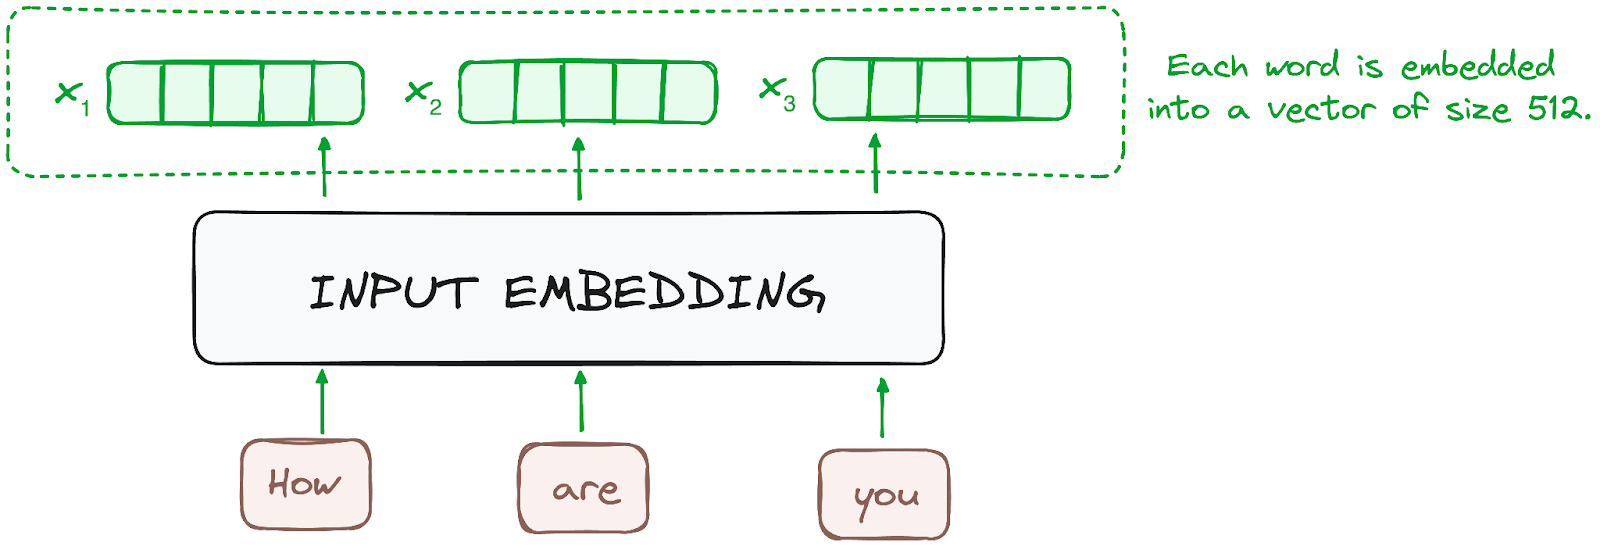
\includegraphics[width=.7\textwidth]{Images/transformer_input_embedding.png}
    \caption{Input embedding of sentence}.
    \label{fig:input_embedding_mechanism}
\end{figure}

There are several ways to represent a sentence as a vector. The simplest one is the one-hot encoding mechanism, 
in which each sentence is represented by a vector with a dimension equal to the vocabulary size, having 1 
if the word is present and 0 otherwise. However, this mechanism does not capture the semantic relationships
between words. What we use in this case is an unsupervised learning method called 
\textbf{Learned Word Embedding}, which learns the semantic relationships within words.
We have mainly two types of word embeddings:
\begin{itemize}
    \item \textbf{Word2Vec}: It is a group of related models that are used to produce word embeddings. 
    These models are shallow, two-layer neural networks that are trained to reconstruct linguistic contexts of 
    words. Word2Vec takes a large corpus of text as its input and produces a vector space, typically of several 
    hundred dimensions, with each unique word in the corpus being assigned a corresponding vector in the space. 
    The vectors are positioned in the vector space such that words that share common contexts in the corpus are located close to one another in the space.
    Examples of Word2Vec are:
    \begin{itemize}
        \item Continous Bag of Words (CBOW)
        \item Skip Gram
    \end{itemize}
    \item \textbf{GloVe}: GloVe (Global Vectors for Word Representation) is an unsupervised learning algorithm for 
    obtaining vector representations for words. Training is performed on aggregated global word-word 
    co-occurrence statistics from a corpus, and the resulting representations exhibit interesting linear 
    substructures of the word vector space. GloVe focuses on the global statistical information of a corpus 
    to learn embeddings by creating word co-occurrence matrices and extracting their statistical information.
\end{itemize}

\paragraph*{CBOW:} The algorithm uses a sliding-windows technique to capture and extract the context of the so 
called \textbf{target words}. For each window in each sentence a target word is picked one by one, 
with the remaining words in the window as context to that target word. The aim of the Neural Network is to 
predict the target word, given the context words. Before passing the input to the NN, we have to pre-process the 
words such that they can be fed into the input layer. Each word $\omega_i$ is represented with a vector 
$v_i \in \mathbb{R}^{V}$ where $V$ is the vocabulary size. Typically, the words are converted into vectors using 
the one-hot-encoding method. The input layer is takes $C$ context words $\{\omega_{t-\frac{C}{2}}, \ldots, \omega_{t-1}, 
\omega_{t+1}, \ldots, \omega_{t+\frac{C}{2}}\}$, with $C$ chosen by the user as hyperparameter and $\omega_t$ being the 
target word. The second layer is called \textbf{projection layer}, in this part the input one-hot-encoded 
vectors are mapped into dense embeddings through a \textbf{embedding matrix} $W \in \mathbb{R}^{V \times D}$, with 
$D$ \textbf{representing the dimensionality of the embeddings chosen as hyperparameter}. For a context word $\omega_j$, the associated 
embedding is calculated as:
\begin{equation} 
    e_j = W^T v_j \text{with } e_j \in \mathbb{R}^{D}
\end{equation}

The \textbf{context vector} $h \in \mathbb{R}^{D}$ is obtained by averaging the embeddings of the context words. This vector is then 
used to predict the final target word. To compute the target word from $h$ we apply the product between a 
\textbf{output embedding matrix} $M \in \mathbb{R}^{D \times V}$ and $h$:
\begin{equation}
    u = M h, \text{with } u \in \mathbb{R}^{V}
\end{equation} 
Through a \textbf{softmax activation function we can convert $u$ into probabilities} for getting a specific word in the 
vocabulary.

\begin{figure}
    \centering
    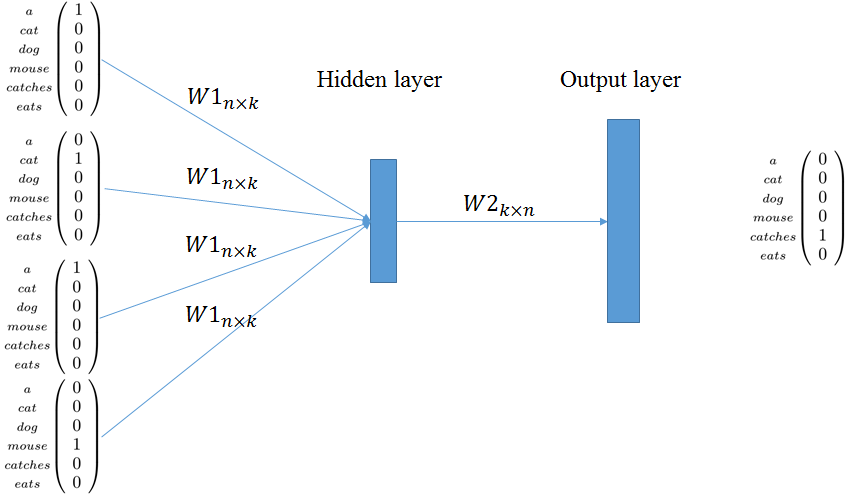
\includegraphics[width=.7\textwidth]{Images/cbow.png}
    \caption{CBOW's model architecture}.
    \label{fig:cbow}
\end{figure}

\subsection{Transformer Encoder}
The \textbf{main goal of the encoder is to transform the input tokens into contextualized representations}. 
Unlike other models, the \textbf{transformer's encoder can capture the context of each token with respect to 
the entire input}. This means the context of each word in the input sentence is dependent on all the other 
words in the sentence. This ability allows the transformer to process multiple inputs in parallel, making 
it suitable for parallel computing offered by GPUs.

As mentioned earlier, the encoding block can consist of more than one \textbf{encoding layer}, each taking 
the output of the previous encoding layer as input. \textbf{All the encoding layers take as input a 512 
fixed-sized numerical vector}. Each encoding layer is structured as shown in 
\hyperref[fig:transformer_encoder]{Figure~\ref*{fig:transformer_encoder}}.

\begin{figure}
    \centering
    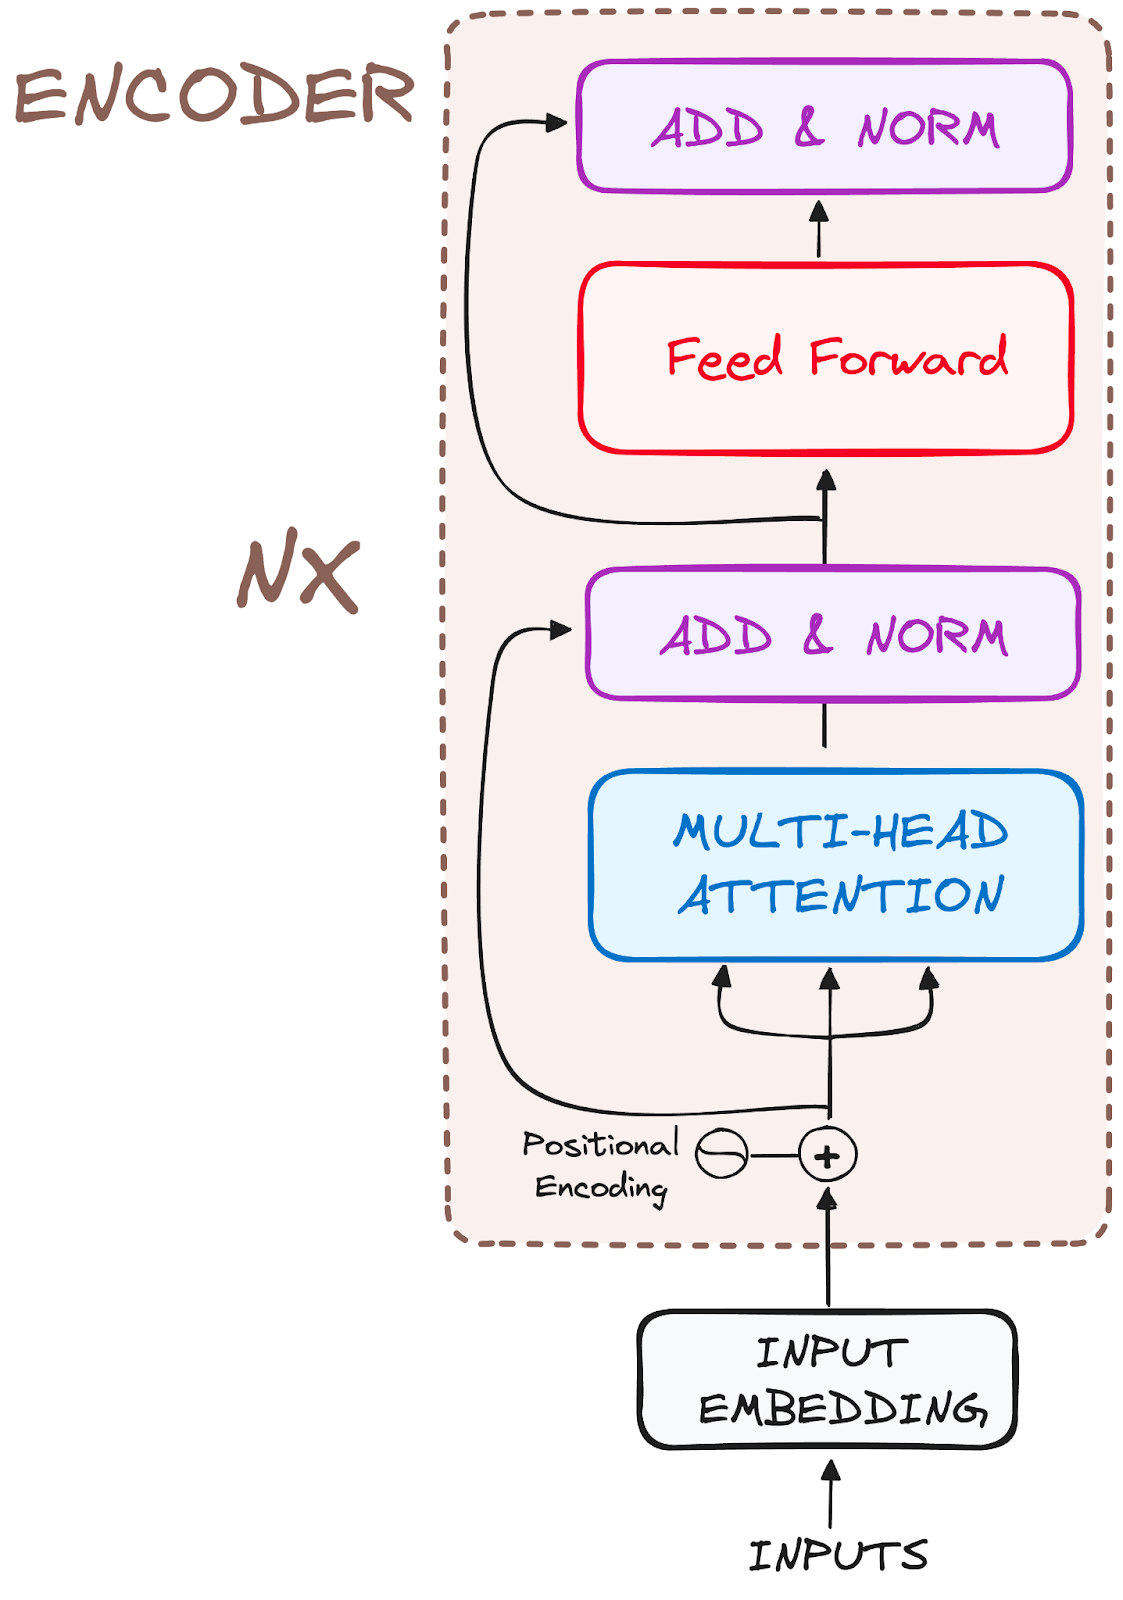
\includegraphics[width=.4\textwidth]{Images/transformer_encoder_architecture.png}
    \caption{Transformer's Encoder architecture}.
    \label{fig:transformer_encoder}
\end{figure}

\subsection{Positional Embeddings}
The input embeddings do not take into account the position of the words in the sentence. This information is 
then introduced in the \textbf{positional encoding step}. To ensure that each position has a unique 
representation, the original paper proposed combining sine and cosine functions to generate a unique vector
representing the position. Considering $L$ as the maximum number of vectors (positions), for each positional 
encoding vector, we loop through the elements two by two, setting the even element to $PE(k, 2i)$ and the 
odd element to $PE(k, 2i + 1)$, with $PE$ defined as follows:

\begin{equation}
    \begin{aligned}
        PE_{(pos, 2i)} &= \sin \left( \frac{pos}{n^{\frac{2i}{d_{\text{model}}}}} \right) \\
        PE_{(pos, 2i+1)} &= \cos \left( \frac{pos}{n^{\frac{2i}{d_{\text{model}}}}} \right)
    \end{aligned}
    \label{eq:transformer_positional_encoding}
\end{equation}    

Here, $n$ is typically chosen to be 10,000, $d_{\text{model}}$ is the embedding dimension, $pos$ is 
the position of the token in the sequence, and $i$ is the index of the element in the positional encoding 
vector. In other words, for each positional encoding vector, for every two elements, we set the even element 
equal to $PE(k, 2i)$ and the odd element equal to $PE(k, 2i + 1)$, for 
$i = 0 \ldots \frac{d_{\text{model}}}{2}$. Each positional encoding vector has a dimensionality equal 
to $L$, with $L$ indicating the highest position in the input (e.g., if we are processing sentences of 
10 tokens, then $L = 10$). 

The \textbf{positional embedding vector and the word embedding vector ad summed up} obtaining the \textbf{word embedding with 
positional context}.

Considering $P$ as the $n \times D$ matrix containing the positional embeddings, 
$p_i$ as the $i^{\text{th}}$ row of $P$, $E$ as the $n \times D$ matrix containing the input sequence embedding and 
$e_i$ as the $i^{\text{th}}$ row of $E$ indicating the $i^{\text{th}}$ token:
then:
\begin{equation}
    E_{pos} = [e_0 + p_0; e_1 + p_1; \dots ; e_n + p_n] \text{ considering ; as the concatenation operation}
\end{equation}
Trivally, $E_{pos} \in \mathbb{R}^{n \times D}$.

\subsubsection{Encoding Layer}
The encoding layer is the building block of the whole encoder. Each encoding layer is composed by two sub-modules:
\begin{itemize}
    \item \textbf{Multi-Head Attention}
    \item \textbf{Fully Connected Layer}
\end{itemize}

\subsubsection{Multi-Head Attention Layer}
\label{subsubsec:transformer_encoder_multi_head} 
The multi-headed attention utilizes a specialized attention mechanism 
known as self-attention. This approach enables the models to relate each word in the input with other words.
The attention score is calculated based on:
\begin{itemize}
    \item \textbf{Query}: A vector that represent a specific token from the input sequence. It represents the current token for which 
    we want to determine how much attention to pay to the other tokens in the sequence.
    \item \textbf{Key}: A vector representation of a token from the input sequence. Keys are used to match with the query to determine 
    the relevance of each token in the sequence to the current token (query).
    \item \textbf{Value}: A value is a vector associated with each token in the input sequence.
    It contains the actual information that will be used to construct the output of the attention mechanism.
\end{itemize}

\begin{figure}
    \centering
    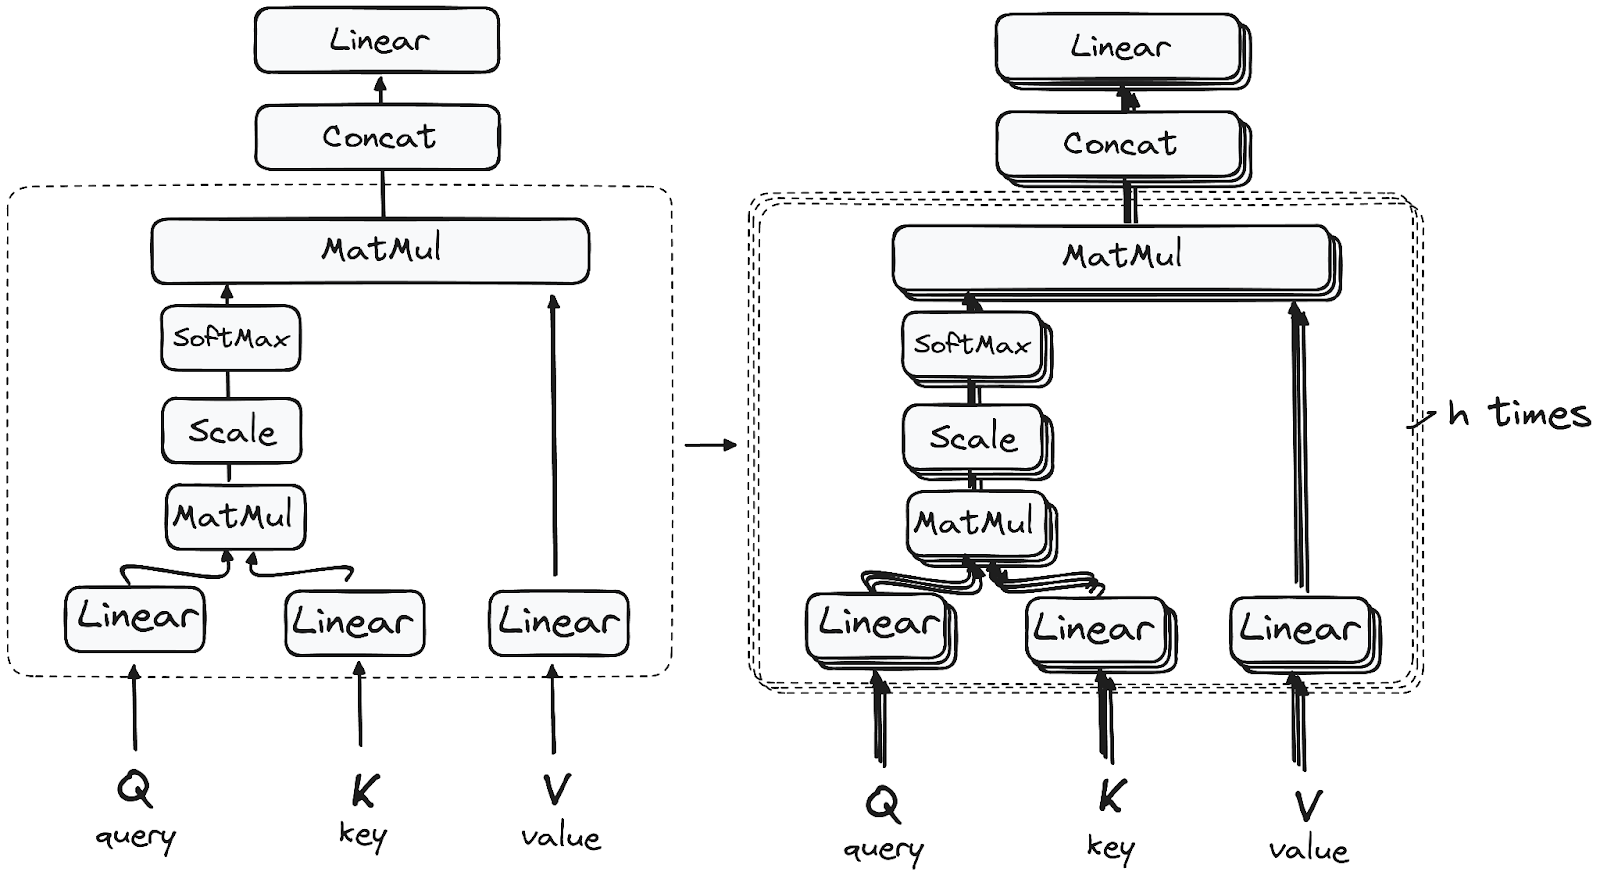
\includegraphics[width=.7\textwidth]{Images/transformer_multi_headed_attention_layer.png}
    \caption{Multi-Headed Attention Layer architecture in detail.}.
    \label{fig:transformer_multi_headed_attention_layer}
\end{figure}

Each Multi-Head Attention Layer is composed of multiple units as shown in 
\hyperref[fig:transformer_multi_headed_attention_layer]{Figure~\ref*{fig:transformer_multi_headed_attention_layer}}:
\begin{enumerate}
    \item \textbf{Linear Projection Layer}: The input sequence embeddings are passed through these layers that 
    will linearly project these embeddings into queries, keys, and values in each of the $h$ heads (where 
    $h$ is an hyperparameter of the model).
    (\hyperref[fig:multi_head_linear_projection_layer]{Figure~\ref*{fig:multi_head_linear_projection_layer}}). 
    Mathematically:
    \begin{equation}
        \begin{aligned}
            Q_i &= X \cdot W_Q^i + b_Q^i \\
            K_i &= X \cdot W_K^i + b_K^i \\
            V_i &= X \cdot W_V^i + b_V^i
        \end{aligned}
        \label{eq:multi_head_attention_linear_projection_single_head}
    \end{equation}
    With $X \in \mathbb{R}^{n \times D}$, $W_Q^i, W_K^i, W_V^i \in \mathbb{R}^{D \times \frac{D}{h}}$, 
    $Q_i, K_i, V_i \in \mathbb{R}^{n \times \frac{D}{h}}$ and $b_Q^i, b_K^i, b_V^i \in \mathbb{R}^{\frac{D}{h}}$
    for the $i^{\text{th}}$ head.

    \textbf{To perform the sum between the matrix obtained though the multiplication and the biases, we 
    perform a row-wise sum}.

    \begin{figure}
        \centering
        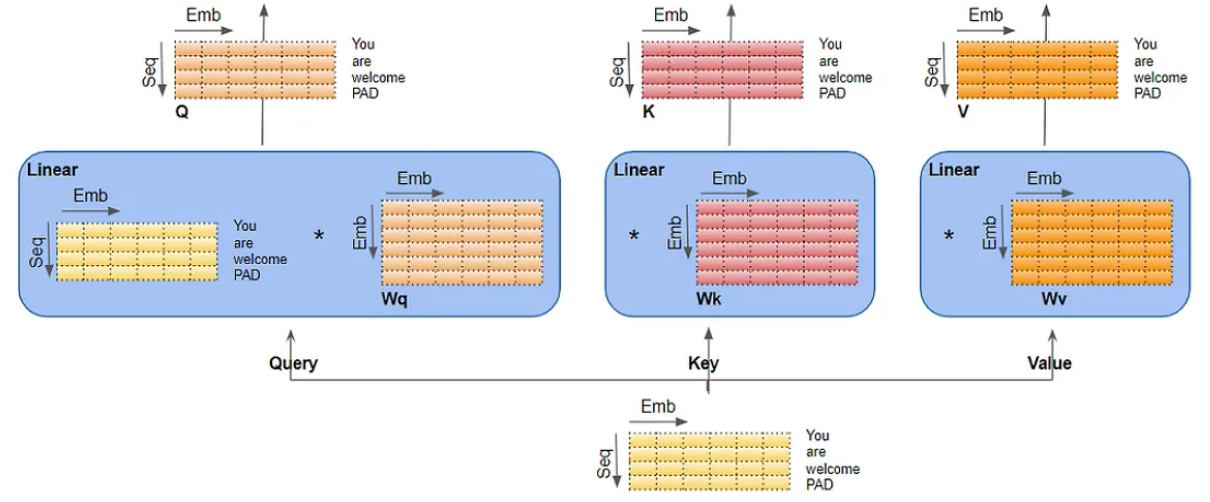
\includegraphics[width=.9\textwidth]{Images/multi_head_linear_projection_layer.png}
        \caption{Linear Projection Layer architecture. As we can see, the resulting matrices $Q, K,$ and $V$ are all
        of the shape $n \times D$ because they are logically split among the heads.}
        \label{fig:multi_head_linear_projection_layer}
    \end{figure}

    \item \textbf{Matrix Multiplication (MatMul) Layer}: This layer simply performs
    a simple matrix multiplication between the query matrix $Q_i$ and the key matrix $K_i$ in each head $i$:
    \begin{equation}
        S_i = Q_i \cdot K_i^T
    \end{equation}
    With $S_i \in \mathbb{R}^{n \times n}$.

    \item \textbf{Scale Layer}: The result $S_i$ is scaled by a $\sqrt{D_k}$ factor, with $D_k = \dfrac{D}{h}$:
    \begin{equation}
        S_i^{scaled} = \dfrac{S_i}{\sqrt{D_k}}
    \end{equation}

    \item \textbf{Softmax Layer}: A softmax activation function is applied to $S_i^{scaled}$ to obtain the 
    attention score. Each score is transformed into a value between 0 and 1, and the sum of all scores for a 
    given query sums to 1:
    \begin{equation}
        \text{Attention Weights}_i = \text{softmax} (S_i^{scaled})
    \end{equation}

    \item \textbf{Second Matrix Multiplication (MatMul) Layer}: The following step of the attention mechanism 
    is that weights derived from the softmax function are multiplied by the value matrix, to achieve the output 
    of the attention mechanism:
    \begin{equation}
        O_i = \text{Attention Weights}_i \cdot V_i
    \end{equation}
    With $O_i \in \mathbb{R}^{n \times \frac{D}{h}}$. 
    
    The whole process described up to now, can be summarized in a single equation:
    \begin{equation}
        \label{eq:transformer_self_attention_score}
        O_i = \text{softmax} \left( \dfrac{Q_i \cdot K_i^T}{\sqrt{d_k}} \right) V_i
    \end{equation}

    \item \textbf{Concatenation Layer}: The single head's scores are then merged into a single score table 
    $A \in \mathbb{R}^{n \times D}$:
    \begin{equation}
        A = [O_0; O_1; \dots; O_h]
    \end{equation}

    \item \textbf{Linear Projection Layer}: The obtained matrix $A$ is then projected using a trainable matrix 
    $W \in \mathbb{R}^{D \times D}$ and $b \in \mathbb{R}^D$:
    \begin{equation}
        A^* = A \cdot W + b
    \end{equation}
    With $A^* \in \mathbb{R}^{n \times D}$.
\end{enumerate}

\subsubsection{Normalization and Residual Connections}
\label{subsubsec:transformer_normalization_layer}
Each sub-layer in an encoder layer is followed by a normalization step. Also, each sub-layer's output is 
added to its input (\textbf{residual connection}) to help mitigate the vanishing gradient problem, allowing deeper 
models (\hyperref[fig:transformer_encoder_add_residual]{Figure~\ref*{fig:transformer_encoder_add_residual}}). 

\begin{figure}
    \centering
    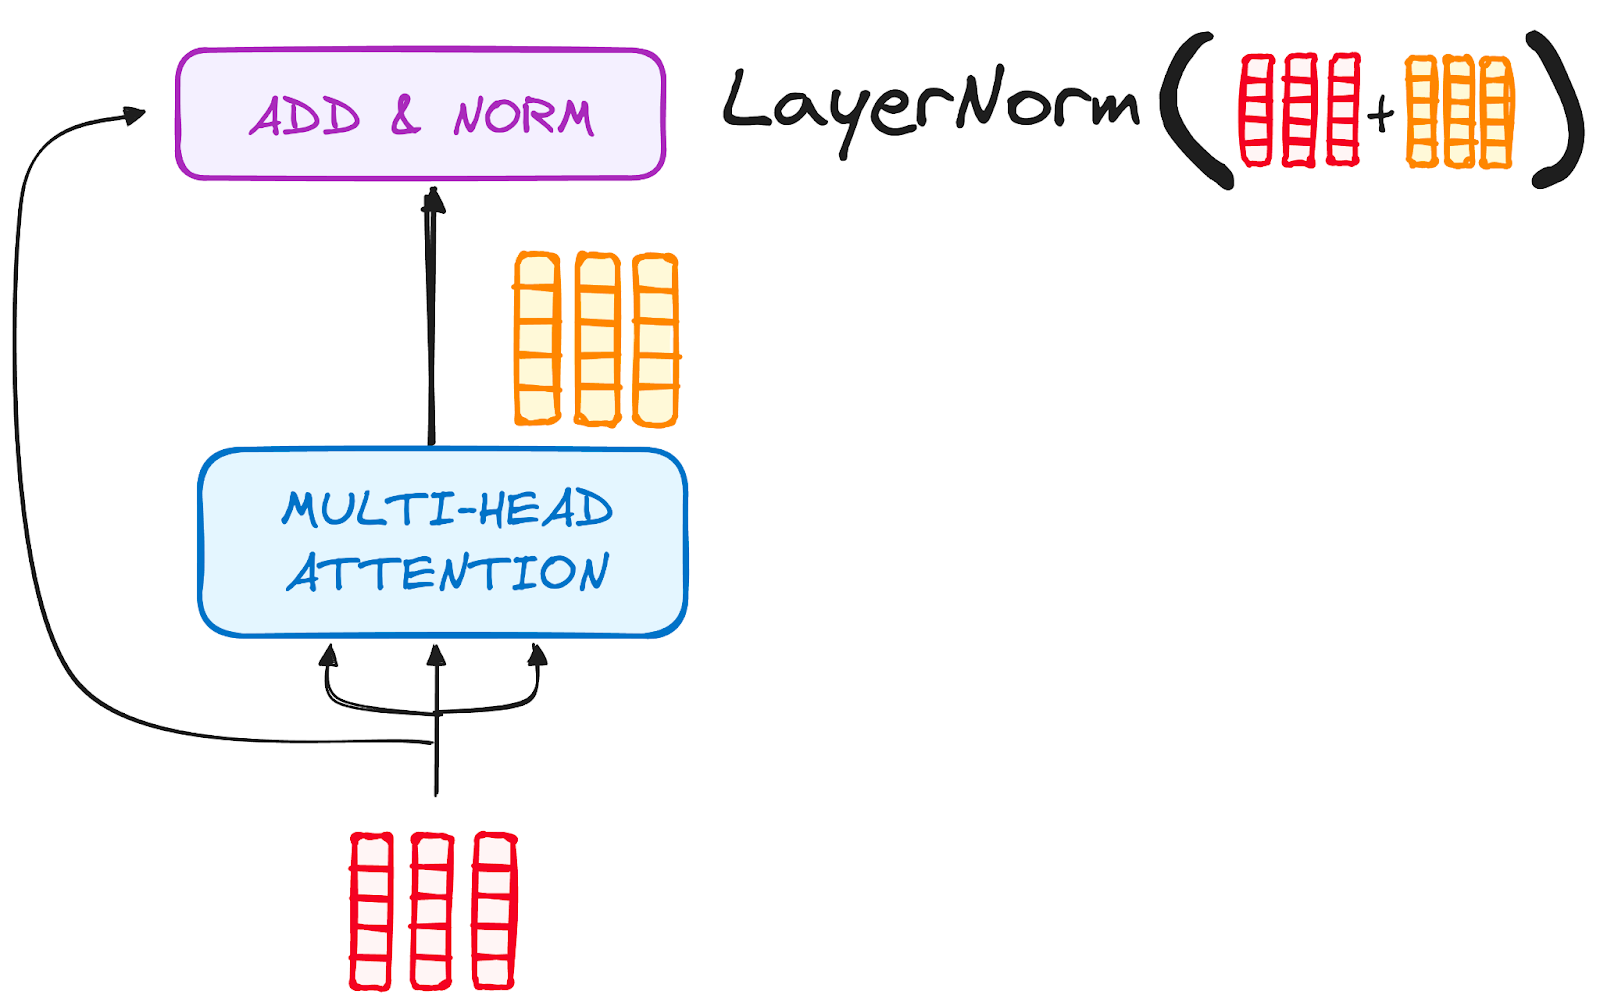
\includegraphics[width=.4\textwidth]{Images/transformer_encoder_add_residual.png}
    \caption{}
    \label{fig:transformer_encoder_add_residual}
\end{figure}

\subsubsection{Feed-Forward Network}
\label{subsubsec:transformer_encoder_feed_forward}
The FFN is composed of a linear projection layer, a ReLU\footnote{ReLU is an activation function defined 
as $ReLU(x) = \max(0, x)$} and another linear projection layer 
(\hyperref[fig:transformer_encoder_ffn]{Figure~\ref*{fig:transformer_encoder_ffn}}). This layer is again 
followed by a normalization and residual layer.

Mathematically, given an input matrix $A^* \in \mathbb{R}^{n \times D}$, the FFN operates as follows:
\begin{enumerate}
    \item \textbf{First Linear Projection}: The first linear transformation is applied to $A^*$ using weight
    matrix $W_1 \in \mathbb{R}^{D \times L}$ and $b_1 \in \mathbb{R}^L$ ($L$ is an hyperparameter of the network):
    \begin{equation}
        Z = A^* \cdot W_1 + b_1 \quad \text{with} \quad Z \in \mathbb{R}^{n \times L}
    \end{equation}

    \item \textbf{ReLU Activation}: The output $Z$ is then passed through the ReLU activation function:
    \begin{equation}
        Z' = \text{ReLU}(Z) \quad \text{with} \quad Z' \in \mathbb{R}^{n \times L}
    \end{equation}

    \item \textbf{Second Linear Projection}: The result $Z'$ is transformed again using weight matrix 
    $W_2 \in \mathbb{R}^{L \times D}$ and $b_2 \in \mathbb{R}^D$:
    \begin{equation}
        O = Z' \cdot W_2 +b_2 \quad \text{with} \quad O \in \mathbb{R}^{n \times D}
    \end{equation}
\end{enumerate}
The final output $O$ from the feed-forward network maintains the same shape as the input $A$, ensuring 
consistency in the architecture.

Following the feed-forward operation, the output $O$ is then combined with the original input $A$ through a residual connection:
\begin{equation}
    O_{\text{final}} = \text{LayerNorm}(O + A)
\end{equation}


\begin{figure}
    \centering
    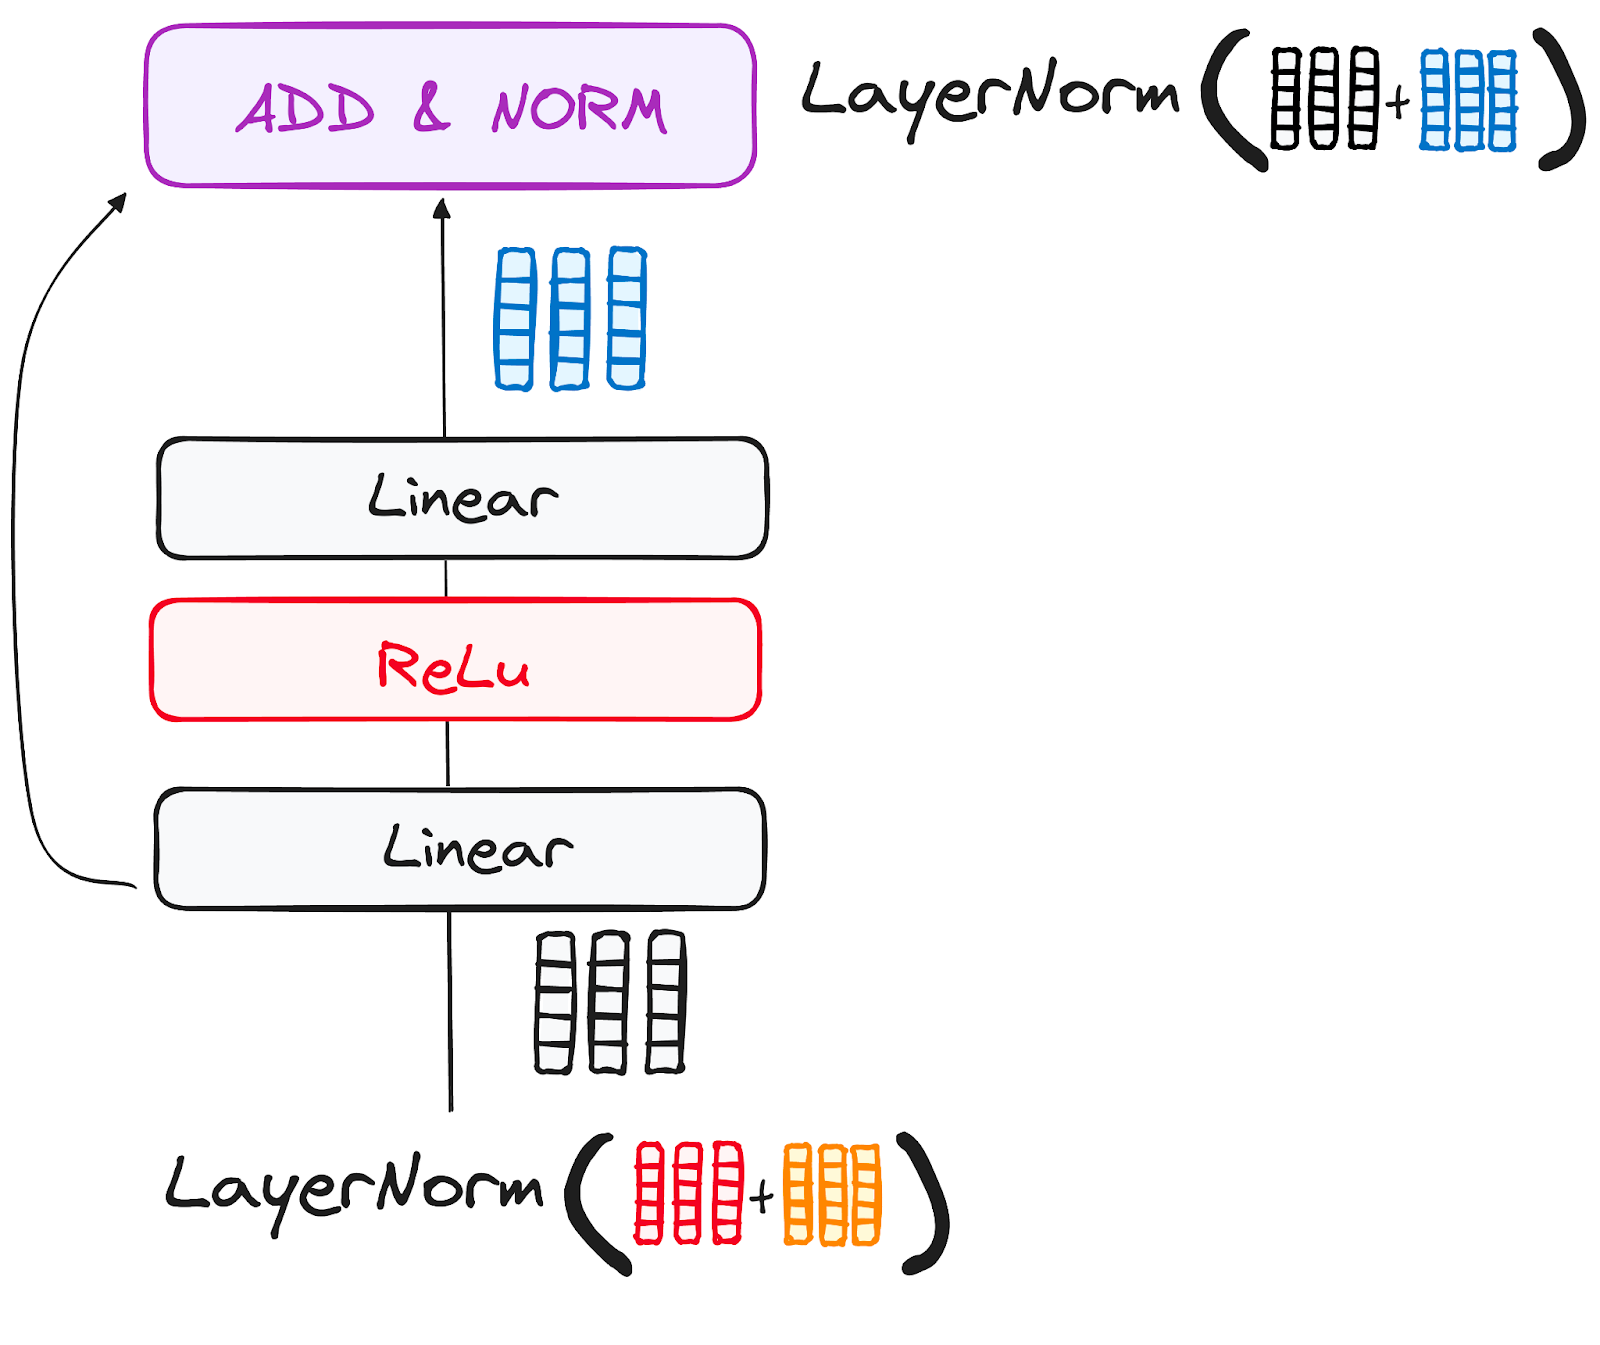
\includegraphics[width=.4\textwidth]{Images/transformer_encoder_ffn.png}
    \caption{}
    \label{fig:transformer_encoder_ffn}
\end{figure}

\subsection{Considerantions about Self-Attention}
The attention mechanism can be also explained from a geometrical point of view. By multiplying the queries with the keys, we are 
likely calculating the cosine similarity between the words (i.e. how much each word match with the other in the dataset). The 
scaling factor is perfomed to stabilize the result, preventing the gradient from fluctations, thus helping the model during the
training. The softmax oparations ensures that the scores are translated into probabilities that when summed up give 1 as result.
Lastly, the values are used to indicate how much the transformer should pay attention to each word in the dataset. 

\subsection{Output Encoding}
The first module encountered after exiting from the last encoder is the output encoding layer. \textbf{The decoder} doesn't 
take as input the output of the last encoder layer; instead, it \textbf{takes the output sequence associated with the 
input sequence given to the encoder} (e.g. We want to train a transformer able to translate a sentence from 
English to Italian; if the encoder takes as input the embeddings of "The pen is blue", the decoder will take 
as input "La penna è blu"). As with the encoding layer, we first have to produce embeddings before feeding the 
sentence to the decoder. This is done through the output encoding layer; it works exactly like the input encoding 
layer.

\subsection{Transformer Decoder}
The decoder's role centers on crafting text sequences. Mirroring the encoder, the decoder is equipped with 
a similar set of sub-layers. It is composed of two multi-head attention layers and a feed-forward layer, all 
of which are intermediated by a residual connection and normalization layer (\hyperref[fig:transformer_decoder_architecture]{Figure~\ref*{fig:transformer_decoder_architecture}}). 
The final output is passed through a linear layer that acts as a classifier, and the result is processed using 
a softmax function that outputs the probability of each word. \textbf{While the encoder is designed to attend to all 
the words in the input sequence, the decoder is modified to attend only to the preceding words; hence, the prediction 
of the next token can only be done based on the previous words}.

\begin{figure}
    \centering
    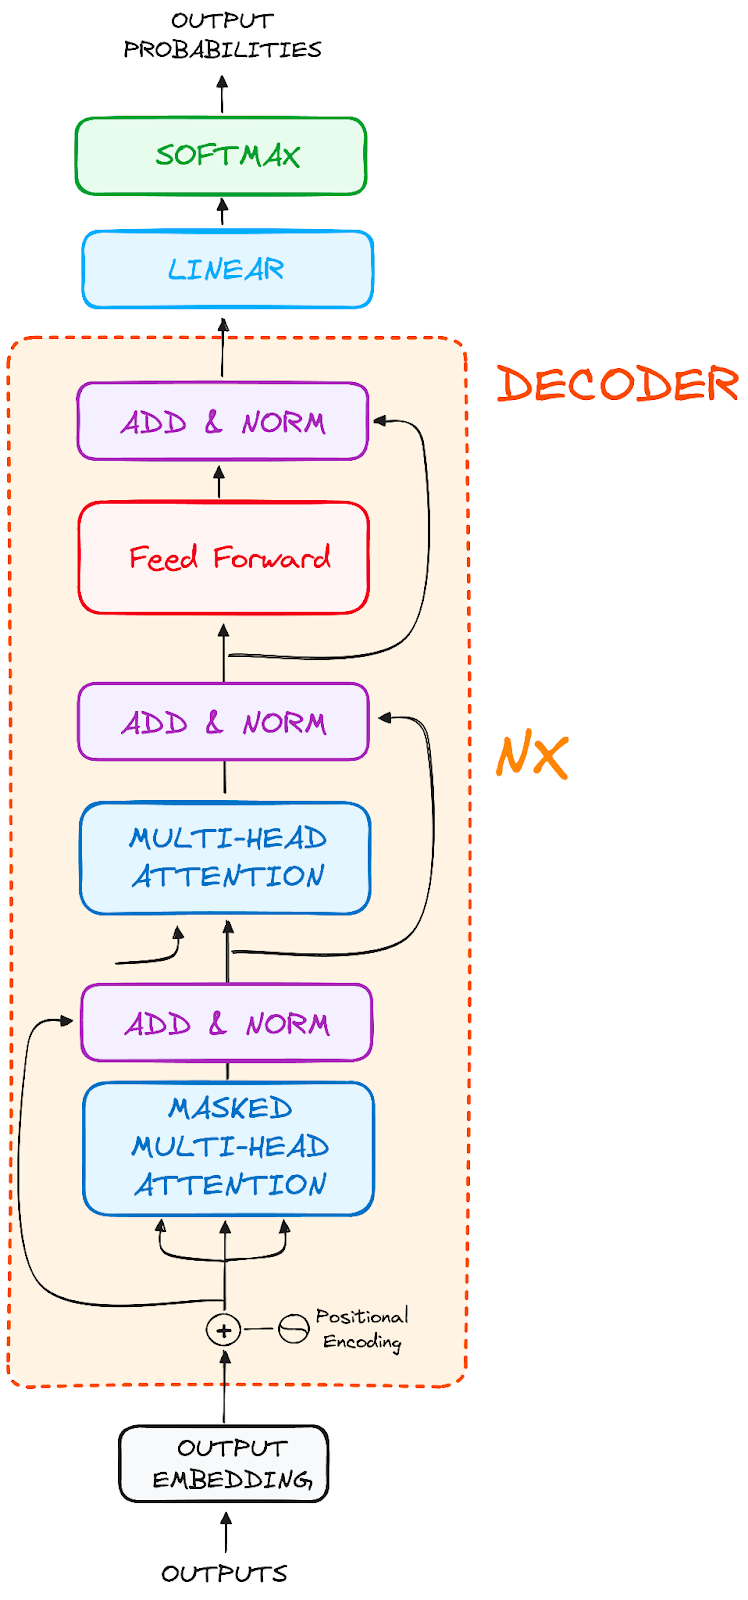
\includegraphics[width=.35\textwidth]{Images/transformer_decoder_architecture.png}
    \caption{Transformer's Decoder architecture}
    \label{fig:transformer_decoder_architecture}
\end{figure}

\subsubsection{Positional Embedding}
Again, even for the decoder, the position matters. Therefore, we combine the embedding given by the output
encoding layer with the positional encodings obtained through the 
\hyperref[eq:transformer_positional_encoding]{Equation~\ref*{eq:transformer_positional_encoding}}.


\subsubsection{Decoding Layer}
The decoder consists of a stack of identical layers (6 in the original Transformer model). Each layer has three 
main sub-components:
\begin{itemize}
    \item \textbf{Masked Self-Attention Mechanism}
    \item \textbf{Encoder-Decoder Multi-Head Attention or Cross Attention}
    \item \textbf{Feed-Forward Neural Network}
\end{itemize}

\subsubsection{Masked Self-Attention Mechanism}
This is similar to the self-attention mechanism in the encoder but with a crucial difference: \textbf{it prevents 
positions from attending to subsequent positions, which means that each word in the sequence isn't influenced 
by future tokens}. The scores are computed through 
\hyperref[eq:transformer_self_attention_score]{Equation~\ref*{eq:transformer_self_attention_score}}, then for each 
row (i.e., word of the output sequence), the scores that are above the diagonal that goes from top-left to bottom-right
are changed to $-\inf$. Namely, only the scores of the words that precede the target word are kept, thus 
preventing the influence from the future word in the sequence (\hyperref[fig:transformer_decoder_self_attention]{Figure~\ref*{fig:transformer_decoder_self_attention}}).
The output of the layer is the score matrix $S^i \in \mathbb{R}^{n \times n}$ in each head $i$.

\begin{figure}
    \centering
    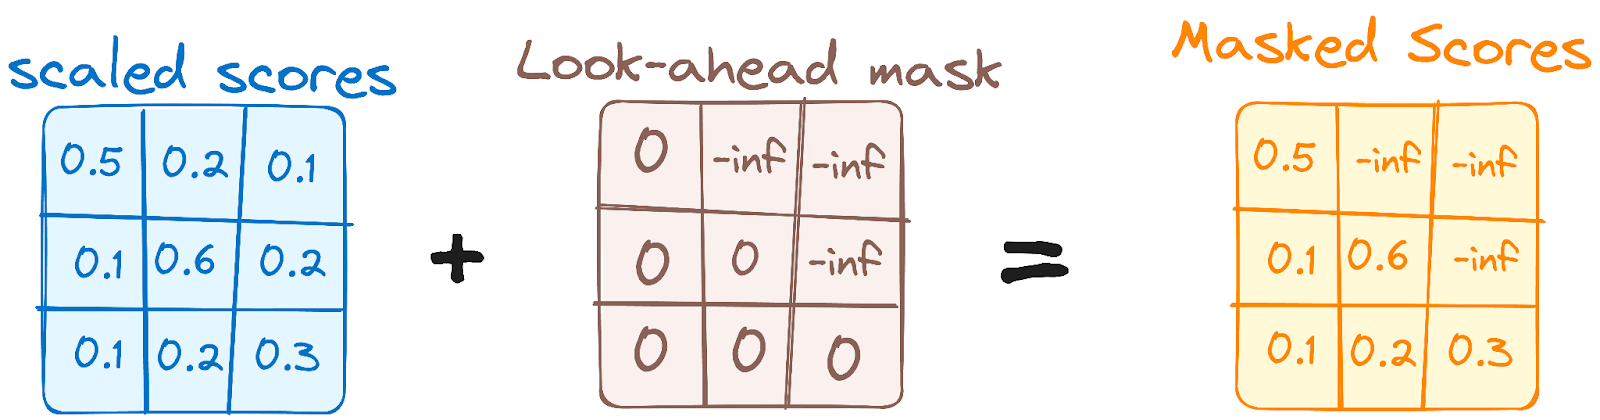
\includegraphics[width=.5\textwidth]{Images/transformer_decoder_self_attention.png}
    \caption{Masked Self-Attention mechanism simplified.}
    \label{fig:transformer_decoder_self_attention}
\end{figure}

\subsubsection{Encoder-Decoder Multi-Head Attention or Cross Attention}
This layer is a multi-head attention layer in which both the encoder and the decoder output are used to 
compute the attention score. Thanks to this, the decoder can learn how the input and the output sequence are 
related to eachother. In detail the last encoder's output is $S \in \mathbb{R}^{n \times D}$, the masked multi-head layer output 
is also $M \in \mathbb{R}^{n \times D}$, then similarly in \hyperref[eq:multi_head_attention_linear_projection_single_head]{Equation~\ref*{eq:multi_head_attention_linear_projection_single_head}}, 
we compute query, key and value matrices through linear projection layers as follows:
\begin{equation}
    \begin{aligned}
        Q_i &= S \cdot W_Q^i + b_Q^i \\
        K_i &= S \cdot W_K^i + b_K^i \\
        V_i &= M \cdot W_V^i + b_V^i
    \end{aligned}
    \label{eq:decoder_multi_head_attention_linear_projection_single_head}
\end{equation}   
With $W_Q^i, W_K^i, W_V^i \in \mathbb{R}^{D \times \frac{D}{h}}$, and 
$Q_i, K_i, V_i \in \mathbb{R}^{n \times \frac{D}{h}}$ and $b_Q^i, b_K^i, b_V^i \in \mathbb{R}^{\frac{D}{h}}$
for the $i^{\text{th}}$ head. The other steps shown in 
\hyperref[fig:transformer_multi_headed_attention_layer_decoder]{Figure~\ref*{fig:transformer_multi_headed_attention_layer_decoder}}
are exactly like those described in \hyperref[subsubsec:transformer_encoder_multi_head]{Section~\ref*{subsubsec:transformer_encoder_multi_head}}.

\begin{figure}
    \centering
    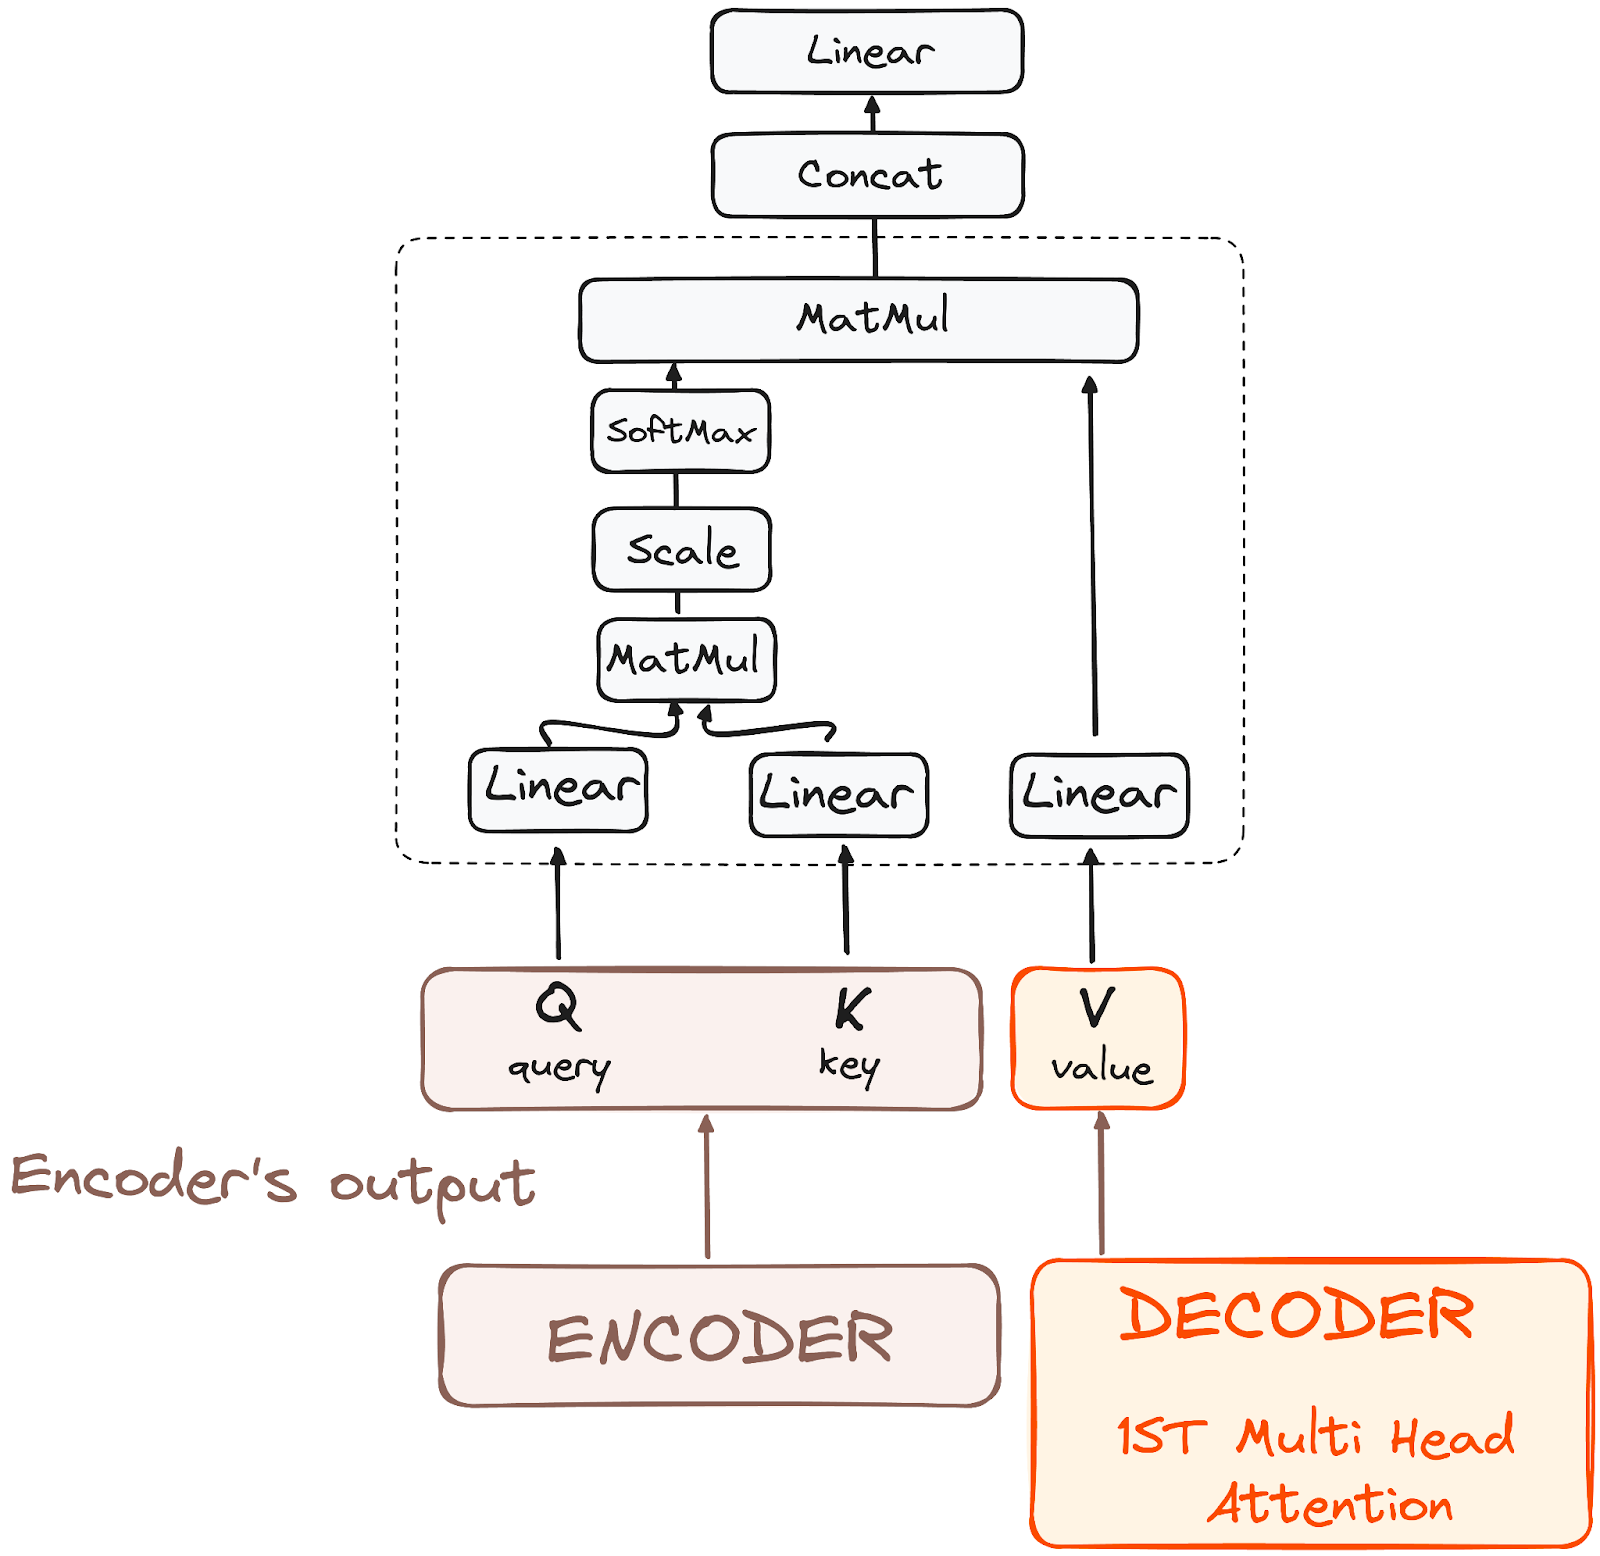
\includegraphics[width=.5\textwidth]{Images/transformer_multi_headed_attention_layer_decoder.png}
    \caption{Multi-head attention layer in the decoding layer. As we can see, the structure of the multi-head attention 
    layer is exactly like the one described in the encoding layer section. The main difference stands in the input 
    provided to it, since we are combining the encoder output and the decoder masked mulit-head layer output.}
    \label{fig:transformer_multi_headed_attention_layer_decoder}
\end{figure}

\subsubsection{Feed-Forward Network}
This part remains exactly like the one described in \hyperref[subsubsec:transformer_encoder_feed_forward]{Section~\ref*{subsubsec:transformer_encoder_feed_forward}}.
The final output is a matrix $O \in \mathbb{R}^{n \times D}$.

\subsubsection{Linear Projection Layer and Softmax Activation Function}
The matrix obtained by the FFN is then passed through a last linear projection layer that projects it into a the 
vocabulary space:
\begin{equation}
    Z_{final} = O \cdot W_{final} + b_{final}
\end{equation}
With $Z_{final} \in \mathbb{R}^{n \times {VocSize}}$, $W_{final} \in \mathbb{R}^{D \times {VocSize}}$ and 
$b_{final} \in \mathbb{R}^{VocSize}$, considering $VocSize = $ vocabulary size. 
Thanks to that we can apply the softmax function to the $Z_{final}$ obtaining the matrix $P \in \mathbb{R}^{n \times {VocSize}}$:
\begin{equation}
    P = \text{softmax}(Z_{final})
\end{equation}
Each row $j$ contains the probability that a word $i$ (i.e. represented by the column $i$) is in the $j^{\text{th}}$
position in the output sequence.

\subsection{Loss}
\label{subsec:transformer_loss}
In the classical transformer architecture, the general loss used is the \textbf{cross-entropy loss}:
\begin{equation}
    \mathcal{L} = - \sum_{N}^{i=1} y_i \log (\hat{y}_i)
\end{equation}
Where $N$ is the number of classes (i.e. vocabulary size), $y_i$ is the is the true distribution (often one-hot encoded) of the target class
and $\hat{y}_i$ is the predicted probability of the class. 




\section{Vision Transformer (ViT)}
The original transformer treated in \hyperref[sec:transformer]{Section~\ref*{sec:transformer}} was designed 
for NLP tasks. However, the Vision Transformer achieved, when released, highly competitive results in many 
computer vision tasks such as image classification, object detection, and semantic image segmentation, hence 
outperforming CNN-based methods with lower computing capability needs.
The original ViT architecture was released in late 2020.

The original ViT architecture (\hyperref[fig:vit_architecture]{Figure~\ref*{fig:vit_architecture}}) 
is very similar to the classical Transformer architecture:
\begin{itemize}
    \item \textbf{Encoder}
    \item \textbf{Classifier}
\end{itemize}

\begin{figure}
    \centering
    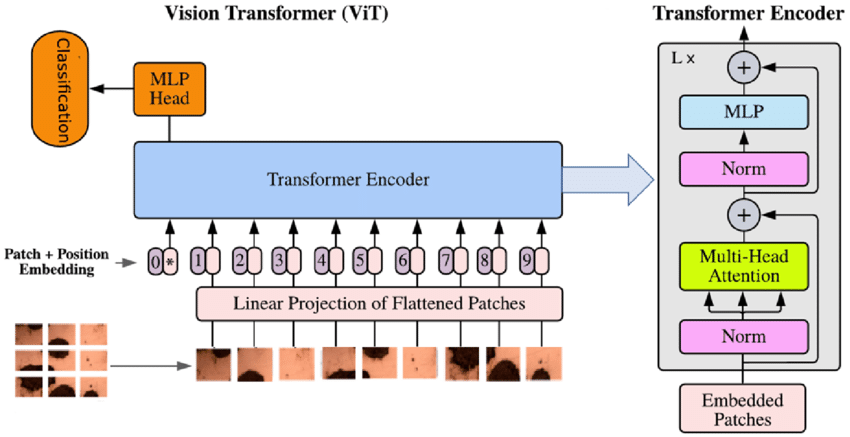
\includegraphics[width=.85\textwidth]{Images/vit_architecture.png}
    \caption{Vision Transformer (ViT) original architecture.}
    \label{fig:vit_architecture}
\end{figure}

\subsection{Input Pre-processing}
Unlike NLP tasks in which we already have an implicit splitting in the input, represented by blank spaces 
between words, in computer vision tasks the input is typically an image. Therefore, a pre-processing step is 
needed to produce an input that can be fed into the architecture:
\begin{enumerate}
    \item \textbf{Image splitting}: The image is first split into $n$ \textbf{square patches}, hence smaller pieces of 
    images such that they can be processed easily. The original image has a shape \\$(height, width, channels)$, 
    while each patch $i$ has the shape $(p, p, c)$.
    
    \item \textbf{Patches flattening}: The obtained patches are then flattened, so they are "unrolled" and 
    now can be seen as a single array. Mathematically, the $n$ patches are now $n$ line-vectors of shape 
    $(1, p^2 * c)$ (a line vector can be seen as the transpose of a column vector, hence the shape of a line 
    vector is $1 \times k$ considering that a column vector of shape $k$).

    \item \textbf{Linear Projection}: The flattened patches are then linearly projected through an embedding 
    matrix $E \in \mathbb{R}^{(p^2 * c) \times D}$ and $b \in \mathbb{R}^D$, where $D$ is the hyperparameter indicating the 
    embedding size:
    \begin{equation}
        y_i = x_i \cdot E + b
    \end{equation}
    With $x_i$ as the flattened patch, $y_i \in \mathbb{R}^{1,D}$ as the embedded patch (trivially $y_i$ is a line 
    vector). Now we have $n$ embedded patches $(y_0, \dots, y_n)$.

    \item \textbf{Learnable class token add}: An extra learnable class token of shape $(1,D)$ is put at the start of 
    the sequence, resulting in having $n+1$ embedded input tokens of shape $(1,D)$. So we can also see them as 
    a single input matrix $I \in \mathbb{R}^{(n+1) \times D}$. During the self-attention mechanism in 
    ViT, the class token attends to all other patch tokens. This allows it to gather information from all 
    parts of the image. At the final layer of the Transformer, the class token contains a summary of the image's features, 
    which is then used for classification.

    \item \textbf{Positional Embedding}: Like the original transformer, to keep track of positional information, 
    we add to the input matrix $I$ a positional embedding tensor $E_{pose} \in \mathbb{R}^{(n+1) \times D}$.
\end{enumerate}
At the end of the day, our input sequence $Z_0$ is a $(n+1) \times D$ tensor.

\subsection{ViT Encoder}
The encoder is built of different layers, mainly 3:
\begin{itemize}
    \item \textbf{Normalization and Residual Connections Layer (Norm Layer)}.
    \item \textbf{Multi-head Attention Network (MAH or MSP)}.
    \item \textbf{Multi-Layer Perceptrons (MLP)}.
\end{itemize}

\subsubsection{Multi-head Attention Network (MAH or MSP)}
The overall MAH layer architecture remains unchanged with respect to the one presented in 
\hyperref[subsubsec:transformer_encoder_multi_head]{Section~\ref*{subsubsec:transformer_encoder_multi_head}}
and shown in \hyperref[fig:transformer_multi_headed_attention_layer]{Figure~\ref*{fig:transformer_multi_headed_attention_layer}}:
\begin{enumerate}
    \item \textbf{Linear Projection Layers}: Through 3 different linear projection layers, the input matrix $Z_0$
    is projected into 3 different sub-spaces: queries, keys, and values in each $i^{\text{th}}$ head of the $h$ heads:
    \begin{equation}
        \begin{aligned}
            Q_i &= Z_0 \cdot W_Q^i + b_Q^i \\
            K_i &= Z_0 \cdot W_K^i + b_K^i \\
            V_i &= Z_0 \cdot W_V^i + b_V^i
        \end{aligned}
    \end{equation} 
    with $W_Q^i, W_K^i, W_V^i \in \mathbb{R}^{D \times D_h}$ ($D_h = \dfrac{D}{h}$), 
    $Q_i, K_i, V_i \in \mathbb{R}^{(n+1) \times D_h}$ and $b_Q^i, b_K^i, b_V^i \in \mathbb{R}^{\frac{D}{h}}$.

    \item \textbf{MatMul Layer, Scaling Layer, Softmax Layer}: Queries and keys in each head are then multiplied, 
    and the result of the multiplication is scaled by a factor of $\sqrt{D_h}$. Then, the softmax function is applied. 
    The process can be summarized in a single equation: 
    \begin{equation}
        A_i = \text{softmax} \left( \dfrac{Q_i \cdot K_i^T}{\sqrt{D_h}} \right)
    \end{equation}
    with $A_i \in \mathbb{R}^{(n+1) \times (n+1)}$.

    \item \textbf{MatMul Layer (Self-attention Score Calculation)}: The obtained matrix $A_i$ is then multiplied 
    by the value matrix $V_i$ to obtain the self-attention score matrix:
    \begin{equation}
        S_i = A_i \cdot V_i
    \end{equation}
    with $S_i \in \mathbb{R}^{(n+1) \times D_h}$.

    \item \textbf{Concatenation Layer}: All the single score matrices $S_i$ stored in the individual heads are then merged 
    into a single matrix $S \in \mathbb{R}^{(n+1) \times D}$.

    \item \textbf{Linear Projection Layer}: The score matrix $S$ is then projected using a trainable matrix 
    $W_f \in \mathbb{R}^{D \times D}$ and $b_f \in \mathbb{R}^{D}$:
    \begin{equation}
        S^* = S \cdot W_f + b_f
    \end{equation}
    with $S^* \in \mathbb{R}^{(n+1) \times D}$.
\end{enumerate}

\subsubsection{Residual Connections and Norm Layer}
Betweem each sub-module in the encoder, there is a Norm Layer in which the output is summed up with the 
original input (residuals) and then normalized. The goal of this layer is straightforward; it \textbf{normalizes the input values}, thus preventing issues like \textbf{vanishing or exploding 
gradients} and trivially helping the training process. Namely, the Norm Layer ensures that the values are 
equally distributed within the normalization ranges. We have two Norm Layers in the encoder: one positioned 
as the first layer of the encoder module, and the second positioned after the MAH layer:
\begin{equation}
    \text{LayerNorm}(x + \text{Residual}(x))
\end{equation}

\subsubsection{Multi-Layer Perceptrons (MLP)}
The MLP layer is very exactly like the FFN (\hyperref[subsubsec:transformer_encoder_feed_forward]{Section~\ref*{subsubsec:transformer_encoder_feed_forward}}),
with the only difference that the ReLU activation function is replaced with a GELU\footnote{The Gaussian Error 
Linear Unit (GELU) is an activation function used in neural networks, including the Vision Transformer (ViT). 
It's designed to provide a more effective alternative to traditional activation functions like ReLU 
(Rectified Linear Unit). The GELU activation function is defined as follows: $\text{GELU}(x)=x * \Phi(x)$, where $\Phi$
is the cumulative distribution function (CDF) of the standard normal distribution. In practice, this is often approximated for computational efficiency:
$\text{GELU}(x) \approx 0.5x \left(1 + \tanh\left[\sqrt{\frac{2}{\pi}} \left(x + 0.044715x^3\right)\right]\right)$. 
Unlike ReLU, which introduces a discontinuity at zero, GELU is smooth and differentiable everywhere, providing a more gradual transition which can be 
beneficial for training deep networks.} activation function. Therefore 
we have two linear projection layer intermediated by the GELU function:
\begin{equation}
    O = \text{GELU}(S^* \cdot W_1 + b_1) \cdot W_2 + b_2
\end{equation}
With $W_1 \in \mathbb{R}^{D \times P}$, $b_1 \in \mathbb{R}^P$, $W_2 \in \mathbb{R}^{P \times D}$, 
$b_2 \in \mathbb{R}^D$ and $O \in \mathbb{R}^{(n+1) \times D}$.

\subsection{ViT Classifier}
In ViT there is no decoder, instead, its final step is the classification step through a \textbf{Fully-Connected 
Layer (FC)}. Only the class token $z_{cls} \in \mathbb{R}^D$ is used, all the other embeddings are trashed out. 
\begin{equation}
    y = z_{cls} \cdot W_{final} + b_{final}
\end{equation}
With $W_{final} \in \mathbb{R}^{D \times C}$, $b_{final} \in \mathbb{R}^C$ and 
$y\in \mathbb{R}^C$ ($C$ = number of classes). The $y$ vector is the logits vector, thanks to this we can apply the 
softmax function achieveing the probability distribution over the classes:
\begin{equation}
    p_i = \dfrac{e^{(y_i)}}{\sum_{j=1}^{C} e^{y_i}}
\end{equation}
Where $p_i$ is the probability of the $i_{\text{th}}$ class.

\subsection{Loss}
The used loss depends on the task in which ViT is used. In image classification tasks, the \textbf{cross-entropy 
loss} described in \hyperref[subsec:transformer_loss]{Section~\ref*{subsec:transformer_loss}} is typically 
a popular choice. In regression tasks, where ViT has to predict continous values, the loss used can be the 
\textbf{mean squared error (MSE)}:
\begin{equation}
    \text{MSE} = \dfrac{1}{n} \sum_{i=1}^{n} (y_i - \hat{y}_i)^2
\end{equation}
Where $n$ is the number of predicted points, $y_i$ is the ground-truth value and $\hat{y}_i$ is the predicted 
value.




\section{Detection Transformer (DETR)}
In DETR, object detection problem is modeled as a direct set prediction problem. It makes the detection pipeline a 
simple end to end unified architecture. The architecture is build upon two main components:
\begin{itemize}
    \item \textbf{Set-based global loss that forces unique predictions via bipartite matching}.
    \item \textbf{Transformer encoder-decoder architecture}.
\end{itemize}
Given an image, the model must predict an unordered set (or list) of all the objects present, each 
represented by its class, along with a tight bounding box surrounding each one. Transformer acts as a 
reasoning agent between the image features and the prediction.

The DETR pipeline is shown in \hyperref[fig:detr_architecture]{Figure~\ref*{fig:detr_architecture}}.

\begin{figure}
    \centering
    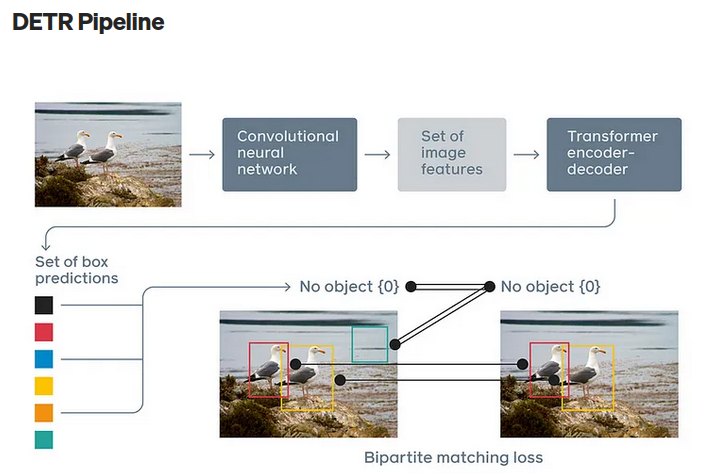
\includegraphics[width=.7\textwidth]{Images/detr_architecture.png}
    \caption{Detection Transformer (DETR) architecture.}
    \label{fig:detr_architecture}
\end{figure}

\subsection{CNN Backbone Module}
DETR both in inference and in training uses a CNN backbone (such as YOLO or ResNet50) to extract a feature representation 
from the input image. This step is used as input embedding step for the transformer architecture. 
Once that the backbone has computed these embeddings, the positional encoding step is applied before fitting
the input to the transformer's encoder (\hyperref[fig:detr_architecture_2]{Figure~\ref*{fig:detr_architecture_2}}).

\begin{figure}
    \centering
    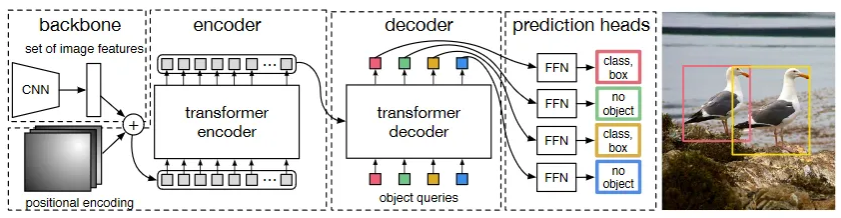
\includegraphics[width=.7\textwidth]{Images/detr_architecture_2.png}
    \caption{Detailed DETR architecture.}
    \label{fig:detr_architecture_2}
\end{figure}

\subsection{Transformer Module}

\subsubsection{DETR Encoder Module}
Once obtained the input features, \textbf{DETR employes a pseudo-classical transformer architecture to calculate the classes and 
bounding boxes}. As we can see from \hyperref[fig:detr_transformer_module]{Figure~\ref*{fig:detr_transformer_module}},
the transformer's encoder takes in input the \textbf{image features provided by the backbone module}. These 
are \textbf{used to calculate the query, key and value matrices} that are then passed through the MAH layer, 
Norm layers and FFN layer. 

\subsubsection{DETR Decoder Module}
The decoder module is slightly changed with respect to the original transformer's decoder. 
Unlike the first-ever transformer design, this model doesn't create the output one step at a 
time (autoregressive). Instead, it processes $N$ objects simultaneously in every decoder layer. These $N$
object are the \textbf{object queries}, they are initialized as a set of \textbf{fixed-size learnable embeddings}. 
Each query can be thought of as an abstract representation or "prototype" that the model learns to 
associate with different object instances during training. This is a fixed number 
(chosen as \textbf{hyperparameter}), if we know that in an input image there can 
be up to 100 objects, then $N$ will be set equal to 100. This number doesn't vary along the images, no matter 
if the objects are more than $N$ (or less than $N$). Each decoder layer has a \textbf{cross-attention mechanism 
where the object queries attend to the last encoder outputs (image features)}.
\textbf{This attention mechanism enables the queries to gather relevant information from different parts of the 
image, helping in precise localization and classification of objects}. The whole decoding process remains 
untouched with respect to the original one.

Since we predict a fixed-size set of $N$ bounding boxes, where N is usually much larger than the actual 
number of objects of interest in an image, an additional special class label $\emptyset$ is used to represent that
no object is detected within a slot. This class plays a similar role to the “background” class in the 
standard object detection approaches.

\begin{figure}
    \centering
    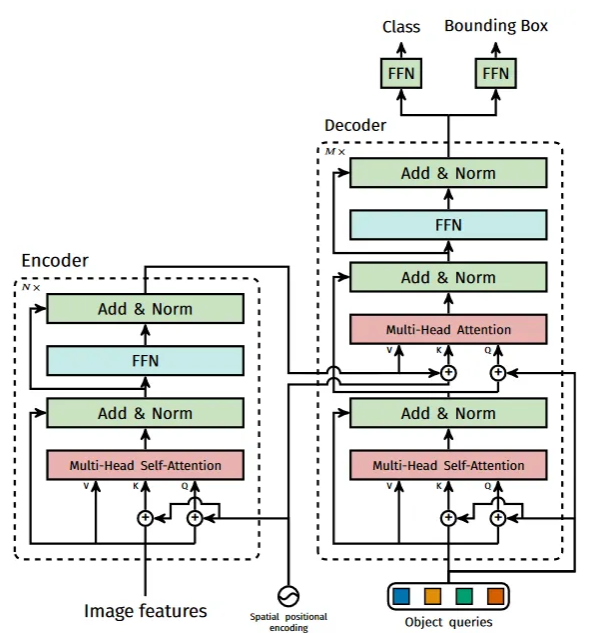
\includegraphics[width=.5\textwidth]{Images/detr_transformer_module.png}
    \caption{DETR Transformer module.}
    \label{fig:detr_transformer_module}
\end{figure}

\subsubsection{DETR Prediction Module}
The final prediction is computed by a 3-layer perceptron with ReLU activation function and hidden dimension $d$, 
and a linear projection layer. The FFN predicts the normalized centercoordinates, height and width of the 
box w.r.t. the input image, and the linear layer predicts the class label using a softmax function.

Each output query is passed though the same FFN and the same linear layer:
\begin{equation}
    \text{FNN Layer}_i(x) = \text{ReLU}(x \cdot W_i + b_i) \text{ with } i=1,\dots,3
\end{equation}
With:
\begin{center}
    $W_1 \in \mathbb{R}^{D \times d}$, $b_1 \in \mathbb{R}^{d}$\\
    $W_2 \in \mathbb{R}^{d \times d}$, $b_2 \in \mathbb{R}^{d}$\\
    $W_3 \in \mathbb{R}^{d \times d}$, $b_3 \in \mathbb{R}^{d}$
\end{center}
Considering as $D$ the input query embedding size.
Let's call $y \in \mathbb{R}^{d}$ the output of the third FNN layer, then the two equations describing 
the linear projection for bounding box predictions 
(\hyperref[eq:detr_bbox_prediction]{Equation~\ref*{eq:detr_bbox_prediction}}) and the class predictions 
are (\hyperref[eq:detr_class_prediction]{Equation~\ref*{eq:detr_class_prediction}}):

\begin{equation}
    \text{Bounding Box} (x) =  y \cdot W_{box} + b_{box}
    \label{eq:detr_bbox_prediction}
\end{equation}
With $W_{box} \in \mathbb{R}^{d \times 4}$, $b_{box} \in \mathbb{R}^4$ (4 because we are predicting
normalized centercoordinates, height and width of the box).

\begin{equation}
    \text{Class} (x) =  y \cdot W_{class} + b_{class}
    \label{eq:detr_class_prediction}
\end{equation}
With $W_{class} \in \mathbb{R}^{d \times C}$, $b_{class} \in \mathbb{R}^C$ (considering as $C$ the number of 
possible classes).




\section{Deformable DETR}
\textbf{Original DETR suffers from slow convergence and limited feature spatial resolution} due to the limitations 
of Transformer attention modules. Deformable DETR was proposed to partially solve these problems by attending 
only to a small set of key sampling points around a reference. In other words, instead of attending to the 
whole image, this implementation focuses attention on small areas. 

In the original attention mechanism, long training sessions are required for the transformer to understand which 
keys are more relevant than others. This can lead to longer training times (more epochs needed to reach convergence)
and worse performance in detecting small objects. 

Deformable DETR is built upon two concepts:
\begin{itemize}
    \item \textbf{Multi-scaled Features}.
    \item \textbf{Deformable Attention Mechanism}.
\end{itemize}

\subsection{Deformable Attention Mechanism}
In the classical DETR implementation, the feature maps are obtained through a ResNet50 model; this is also 
similarly done in the deformable version. However, instead of picking only the output of the last 
ResNet50 block, \textbf{we take the outputs of the last three blocks, resulting in four distinct high-level feature maps
generated by applying convolutional operations}, as shown in 
\hyperref[fig:deformable_detr_multi_scale_feature_maps]{Figure~\ref*{fig:deformable_detr_multi_scale_feature_maps}}. 

\begin{figure}
    \centering
    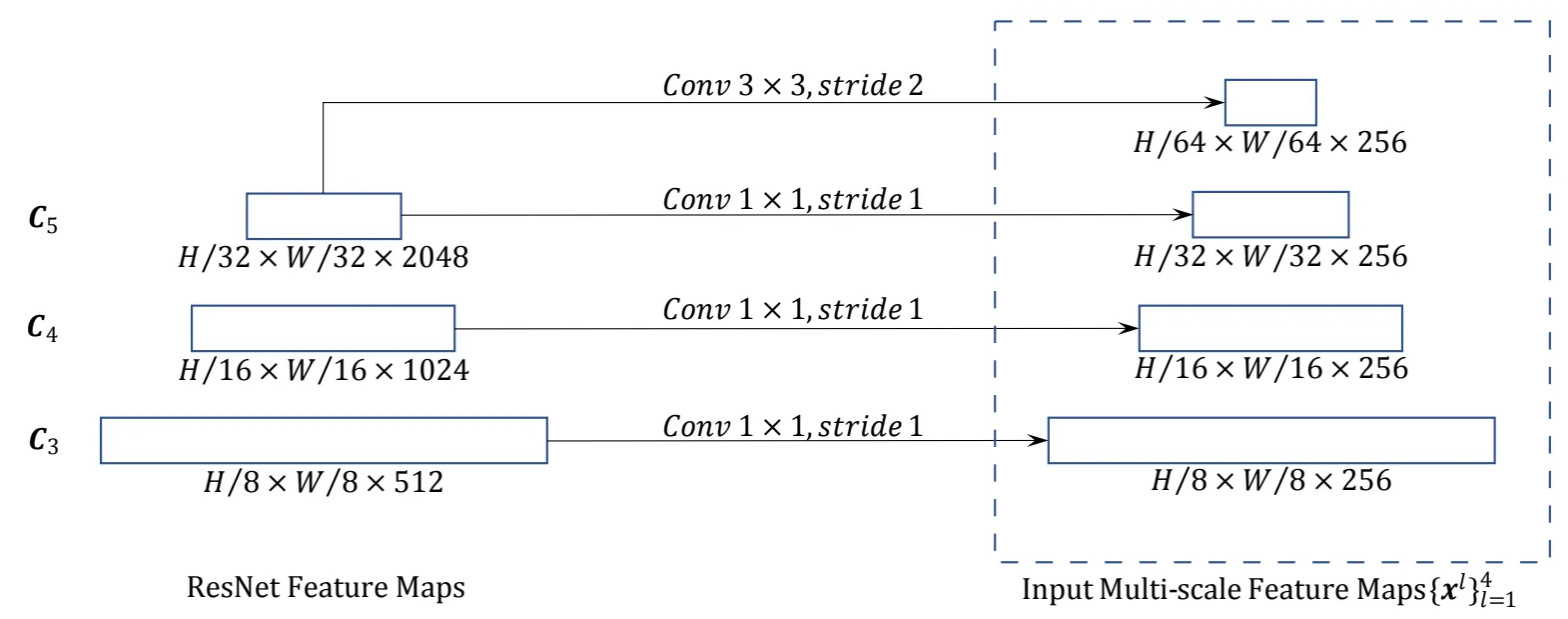
\includegraphics[width=.8\textwidth]{Images/deformable_detr_multi_scale_feature_maps.png}
    \caption{Deformable DETR multi-scale feature maps. On the right side, we have the last three ResNet
    convolutional blocks; the intermediate output is then used to build the multi-scale feature maps on the left 
    side.}
    \label{fig:deformable_detr_multi_scale_feature_maps}
\end{figure}

\subsubsection{Features Maps Flattening}
Exactly like DETR, in deformable DETR these feature maps are flattened and positional encodings are then 
added to them. Consider a backbone network that extracts multi-scale feature maps denoted as:
$\{F_1, F_2, \ldots, F_L\}$ where each $F_l$ has dimensions $C_l \times H_l \times W_l$.
Each feature map $F_l$ is flattened from a 3D tensor to a 2D matrix:

\begin{equation}
    \text{flatten}(F_l) \rightarrow (H_l \times W_l) \times C_l    
\end{equation}
This reshaping converts each feature map into a sequence of feature vectors. 
All flattened feature maps are concatenated to form a single matrix $F$:

\begin{equation}
    F = [\text{flatten}(F_1); \text{flatten}(F_2); \ldots; \text{flatten}(F_L)]    
\end{equation}
The resulting matrix $F$ has dimensions $N \times D$, where:
$N = \sum_{l=1}^{L} H_l \times W_l$ and $D$ is the unified embedding dimension.

\subsection{Deformable Attention Mechanism}
The first architectural modification relies on both encoder and decoder modules, where respectively
the self-attention module and the cross-attention module, have been substituted with the Deformable 
Attention module.

The original multi-head attention mechanism is described in 
\hyperref[eq:transformer_self_attention_score]{Equation~\ref*{eq:transformer_self_attention_score}}, 
the deformable attention is designed to attended to a small set of keypoints around a reference point, 
hence reducing the computational complexity and improving the performance as we are focusing on relevant 
areas:

\begin{equation}
    \text{DeformableAttention}(Q, K, V) = \sum_{m=1}^{M} W_m \sum_{j=1}^{\mathcal{N}_m} A_{mj} V(\phi_{mj})
\end{equation}
Where:
\begin{itemize}
    \item $M$ is the number of attention heads.
    \item $W_m$ are learnable weights for each head.
    \item $\mathcal{N}_m$ is the set of sampling points for head $m $.
    \item $A_{mj}$ are the attention weights for each sampling point.
    \item $\phi_{mj}$ is the transformation function mapping reference points to sampling points.
    It indicates a specific sampling point. Hence $V(\phi_{mj})$, It's not a straightforward 
    multiplication but rather an operation to obtain the values at the spatial locations determined by
    $\phi_{mj}$.
\end{itemize}
In deformable DETR, $Q,K$ and $V$ matrices can be either the same for all the heads (hence there is only 
one linear projection layer instead of one for each head) or not. 

The positions of sampling points are determined using an offset function, which is learnable and depends on 
the input features. This function dynamically adjusts the sampling locations based on the content:
\begin{equation}
    \phi_{mj} = p_0 + \Delta p_{mj}
\end{equation}
Where $p_0$ is the reference point and $\Delta p_{mj}$ is the learned offset for sampling point $j$ 
in head $m$.

The attention weight $A_{mj}$ is computed as:
\begin{equation}
    A_{mj} = \text{softmax}\left(\frac{Q \cdot K(\phi_{mj})}{\sqrt{d_k}} + \text{PE}(\phi_{mj})\right)
\end{equation}
Where $\text{PE}(\phi_{mj})$ is the positional encoding function.

\textbf{The rest of the architecture is exactly the same of the DETR architecture}.

\end{document}
